\documentclass{standalone}
\usepackage{tikz}
\usepackage{pgfplots}
\pgfplotsset{compat=newest}
\usepackage{amsmath}
\usepackage[american]{circuitikz}
\usepackage{cmbright}

\definecolor{myred}{RGB}{170,0,0}
\definecolor{myblue}{RGB}{0,0,220}
\definecolor{mygreen}{RGB}{0,150,0}
\definecolor{myorange}{RGB}{255,127,0}
\definecolor{mybrown}{RGB}{150,75,0}

\begin{document}
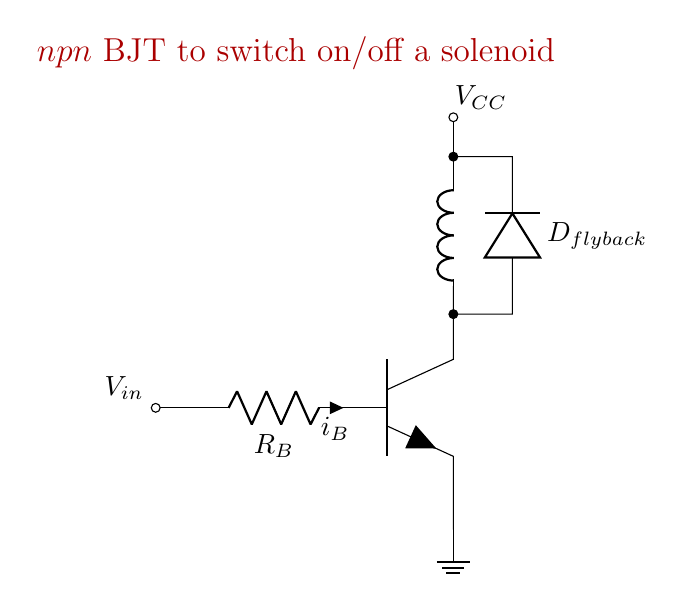
\begin{tikzpicture}
    \begin{scope}
        % Title
        \node[anchor=center, color=myred] at (-2, 3.25) {\large $npn$ BJT to switch on/off a solenoid};
        % npn BJT sumbol
        \draw (0, -1.25) node[npn, scale=2.0] (Q) {};
        \draw ($(Q.base) + (0.4, 0)$)
            to[R, R={$R_B$}, i<={$i_B$}] ++(-2.0, 0)
            to[short, -o, invert] ++(-0.5, 0);
        \node[anchor=center, align=center] at ($(Q.base) + (-2.5, 0.25)$) {$V_{in}$};
        \draw ($(Q.collector) + (0, -0.35)$)
            to[L, *-*, invert] ++(0, 2.0)
            to[short, -o] ++(0.0, 0.5);
        \node[anchor=center, align=center] at ($(Q.collector) + (0.35, 2.4)$) {$V_{CC}$};
        \node[ground] at (Q.emitter) {};
        \draw ($(Q.collector) + (0, -0.35)$)
            to[short, -] ++(0.75, 0.0)
            to[D, l_={$D_{flyback}$}] ++(0, 2.0)
            to[short] ++(-0.75, 0);
    \end{scope}
\end{tikzpicture}
\end{document}